\documentclass[fleqn]{VUMIFPSkursinis}
\usepackage{algorithmicx}
\usepackage{algorithm}
\usepackage{algpseudocode}
\usepackage{amsfonts}
\usepackage{amsmath}
\usepackage{bm}
\usepackage{caption}
\usepackage{color}
\usepackage{float}
\usepackage{graphicx}
\usepackage{listings}
\usepackage{subfig}
\usepackage{wrapfig}

% Titulinio aprašas (nereikalingus elementus užkomentuoti)
\university{Vilniaus universitetas}
\faculty{Matematikos ir informatikos fakultetas}
% \institute{Informatikos institutas}  % Užkomentavus šią eilutę - institutas neįtraukiamas į titulinį
\department{Programų sistemų bakalauro studijų programa}
\papertype{Kursinis darbas}
\title{Migracijos strategijos migruojant iš monolitinės į mikroservisų architektūrą}
\titleineng{Strategies for migrating from monolith to microservices architecture}
\author{Audrius Kumpis}
\status{4 kurso, 2 grupės studentas}
\supervisor{lekt. Vasilij Savin}
\date{Vilnius \\ \the\year}

% Nustatymai
\captionsetup{justification=centering}
% \setmainfont{Palemonas}  % Pakeisti teksto šriftą į Palemonas (turi būti įdiegtas sistemoje)
\bibliography{bibliografija}  % Literatūros šaltinių aprašų failas bus bibliografija.bib

\begin{document}
\maketitle

\tableofcontents

\sectionnonum{Santrauka}
Monolitinės aplikacijos migravimas į mikroservisų architektūrą gali būti itin sudėtingas ir daug planavimo reikalaujantis uždavinys \cite{FBZ+19}. Privaloma atlikti nuoseklų darbų bei būsimo dizaino planavimą, kad migravimas būtų atliktas sėkmingai. Šiame darbe bus palyginti trys metodai, kurių pagalba yra galima atlikti pertvarkymo darbus: dekomponavimas skaidant domenus, visiškas sistemos perdarymas ir dirbtiniu intelektu paremtas įrankis „Mono2Micro“. Metodų lyginimas bus fokusuotas į įvairias metrikas, kaip programinio kodo dydis, priklausomybė nuo padengiamumo funkciniais testais, bei naujos programų sistemos priežiūra. Darbe bus galima pastebėti, jog kiekvienas metodas turi savo pranašumų ir trūkumų, ir kad pats efektyviausias metodas priklausys nuo sistemos specifinių charakteristikų ir reikalavimų, bei nuo trokštamos mikroservisų architektūros dizaino. Darbo metu bus parodyta, jog dekomponavimo pagal domenus ir „Mono2Micro“ metodų kombinacija yra tinkamiausias būdas pertvarkyti monolitinę sistemą. Darbo rezultatas – empiriškai palyginti metodai ir tinkamiausio metodo parinkimas praktiniam realizavimui bakalauro baigiamajame darbe.

\summary{Summary}
The process of refactoring a monolithic application to a microservices architecture can be complex and requires careful planning and design to ensure the success of the migration. In this study, we compare three approaches for refactoring a monolithic application to a microservices architecture: domain-driven design, re-architecture, and the AI tool Mono2Micro. Our evaluation focuses on a variety of metrics, including codebase size, dependency on code coverage, maintainability, and development time. We find that each approach has its own strengths and limitations, and that the most effective approach may depend on the specific characteristics and requirements of the monolithic application and the desired microservices architecture. The results suggest that a combination of domain-driven design and AI-assisted refactoring can be a powerful tool for migrating monolithic applications to microservices, and can help organizations achieve the benefits of a microservices architecture while minimizing the risks and challenges of the refactoring process. Overall result of the article – an empirical evaluation of different approaches and a prepared data for realisation in the Bachelor‘s Thesis.
% \keywords{keyword 1, keyword 2, keyword 3, keyword 4, keyword 5}


\sectionnonum{Įvadas}
Kai komanda pradeda kurti programą, monolitas įprastai yra numatytas pasirinkimas. Tai yra viena pagrindinių priežasčių, kodėl egzistuoja itin daug monolitinių sistemų. Monolitas turi savo duomenų bazę, savo funkcionalumo įgyvendinimą, ir tai yra vientisa programa. Jis yra lengvai suprogramuojamas ir su palyginamai nedideliu darbo indėliu, galima greitai sukurti bei diegti veikiančią sistemą. Tačiau tokią architektūrą yra labai sunku plėtoti bei palaikyti. Kuo daugiau pleti tokią sistemą, tuo daugiau ji didėja, daugėja kodo bei priklausomybių nuo kitų sistemų. Diegimai tampa ilgi ir itin dažni. Testavimas būna sudėtingas, nes negalima atlikti izoliuoto atskirų sistemos modulių testavimo. Kad ši problema būtų išspręsta, paprastai monolitinės sistemos yra skaldomos į mikroservisus. 
Mikroservisai – tai atskiri, nedideli servisai, kurie atsakingi už tam tikras specifines užduotis. Jie yra implementuoti kaip atskiros programos, o komunikacija tarp jų įprastai yra vykdoma per pranešimų siuntimo (angl. messaging) technologijas. Kiekvienas mikroservisas turi savo duomenų bazę, savo diegimo strategijas bei testavimo aplinką. Mikroservisų architektūra išsprendžia šias problemas:
\begin{itemize}
    \item Išskiriami nepriklausomi moduliai.
    \item Pagerinamas sistemos plečiamumas.
    \item Nėra priklausomybės nuo pasirinktų technologijų.
    \item Prie sistemos implementacijos gali dirbti didesnis komandų skaičius.
\end{itemize}

Nors mikroservisai išsprendžia daug problemų, tai nėra paprasta technologija. Kadangi tai yra pilnai techninė užduotis, privaloma gauti projekto vadovo ir/ar projekto savininko sutikimą, kad migracijai būtų skiriami resursai bei lėšos. Sunkiausia migracijos dalis yra mikroservisų projektavimas. Yra daugybė būdų, kaip galima išskaidyti monolitinę sistemą į mažesnius servisus, taigi iš anksto apgalvoti, kokia strategija bus taikoma yra svarbu ir laiko, ir resursų atžvilgiu. Kad migracija iš monolitinės architektūros į mikroservisų būtų sklandi, reikia gerai žinoti, kokius darbus ir kokia tvarka būtina atlikti. Jau egzistuoja keletas migravimo atlikimo strategijų, su kuriomis susipažinus yra lengviau suplanuoti reikiamus darbus. Šiame darbe bus aptartos šios strategijos:
\begin{itemize}
    \item Dekomponavimas skaidant domenus.
    \item Visiškas sistemos perdarymas.
    \item Dekomponavimas naudojant dirbtiniu intelektu paremtą įrankį „Mono2Micro“.
\end{itemize}

\section{Dekomponavimas skaidant domenus}
Pirmiausia aptarsime vieną iš populiariausių migravimo strategijų – skaidymas pagal domenus \cite{Wal22}. Šią strategiją verta naudoti tuomet, kai verslo panaudos sritys yra aiškiai išskirtos. Dažnai  ši sąlyga būna neįgyvendinta, todėl yra itin svarbu į monolito pertvarkymo procesą įtraukti verslo atstovus, analitikus bei kitus techninius sistemos atstovus, kurie gerai nusimano perdaromos sistemos funkcionalume ir esamame įgyvendinime.

\subsection{Strategijos aprašymas}
Dekomponavimas skaidant domenus (angl. domain-driven refactoring) yra viena iš populiariausių migravimo strategijų. Ją labiausiai apsimoka naudoti tuomet, kai monolitas buvo kurtas laikantis domenais remtu kūrimu. Tačiau, ne visada būna taip, jog monolitas yra jau iškarto paruoštas migravimui. Pirmas ir svarbiausias žingsnis yra esminių domenų identifikavimas \cite{LZ22}. Kad esminių domenų identifikavimas būtų atliktas sėkmingai, privaloma įtraukti visus suinteresuotuosius asmenis minėtus anksčiau. Kai domenai yra sėkmingai identifikuoti, belieka juos iškelti į atskirus servisus.


Esminių domenų atskyrimas yra tik dalis darbo. Kai domenai yra identifikuoti, negalima pereiti iškarto prie naujo mikroserviso kūrimo. Jei sekantis žingsnis bus atliktas neteisingai, galima susidurti su funkcionalumo dubliavimusi. Tai yra reiškinys, kai monolite esantis funkcionalumas vis dar gyvuoja šalia naujai sukurto to paties domeno mikroserviso. Tai gali sukelti papildomų problemų ir naudotojams, ir verslui.


Šios problemos sprendimas buvo pristatytas jau 2011 metais, palyginus, mikroservisų idėja buvo pristatyta 2005 metais. Sprendimo idėja yra paprasta: kai naujo domeno funkcionalumas yra įgyvendintas mikroservise ir jau yra paruoštas naudojimui, sistema perima naujojo mikroserviso funkcionalumą ir nebenaudoja jo iš senosios sistemos. Tai yra daroma su kiekvienu esminiu, atrinktu domenu Tokiu būdu, monolitas yra „smaugiamas“ tol, kol jame nebebus nei vieno naudojamo domeno. Iš to ir seka šios taktikos pavadinimas – „Smaugiko šablonas“ \cite{Beh18}. Šis šablonas yra taikomas beveik visuomet, kai yra naudojamas dekomponavimo pagal domenus strategija.

\subsection{Strategijos pritaikymas}
Šiame pavyzdžiui naudosime fiktyvią paskolų išdavimo sistemą. Šioje sistemoje yra naudojami 5 esminiai domenai: autentifikacijos, paskolos dydžio skaičiuoklė, išmokėjimo mechanizmas, kreditingumo skaičiuoklė, transakcijų gavimo mechanizmas. Visi šie domenai veikia darnoje ir yra priklausomi vienas nuo kito. Jų veikimas pavaizduotas šioje diagramoje:
\begin{figure}[H]
    \centering
    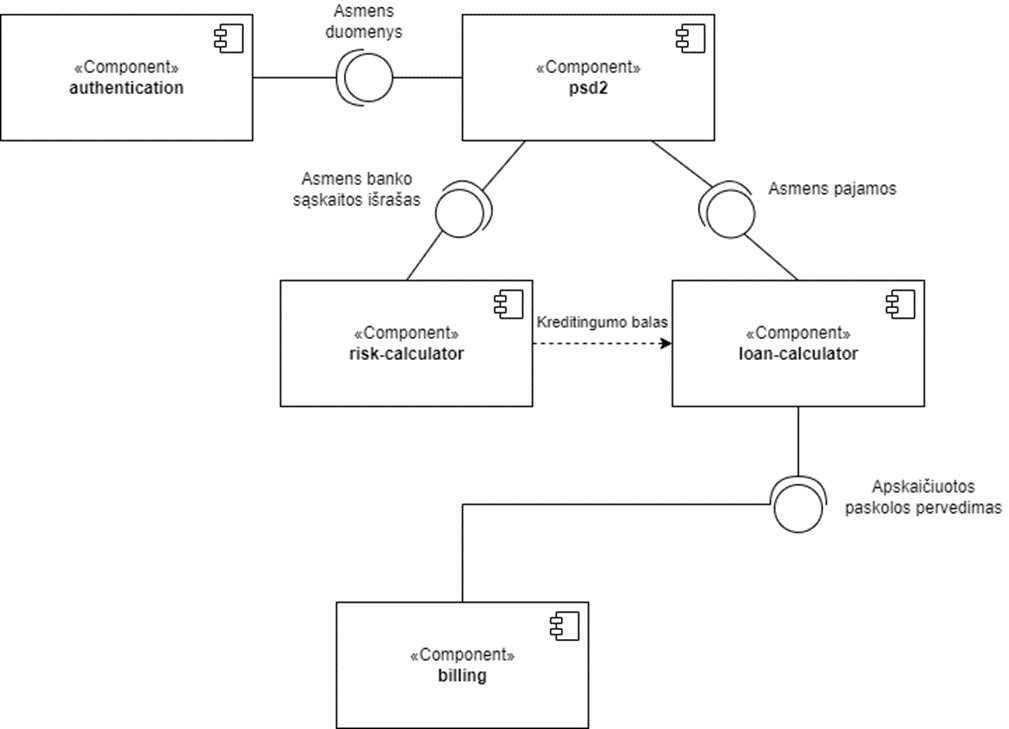
\includegraphics[scale=1.0]{img/komponentu-diagrama.png}
    \caption{Dabartinio monolito komponentų diagrama}
    \label{img:komponentu-diagrama}
\end{figure}

Visi šie domenai – komponentai – priklauso vienas nuo kito. Jei bent vienas neveikia, arba veiks klaidingai, tai atneš nenumatytų nuostolių verslui. Pasinaudojant „smaugiko“ šablonu, iteratyviai kiekvienam išskirtam domenui, sukuriame po mikroservisą. Kūrimo metu, užtikriname, jog bendras sistemos veikimas nėra sugadinamas, jog sistema vis dar veikia korektiškai. Kad tai būtų užtikrinta, privaloma kuo anksčiau sukonfigūruoti pastovaus diegimo/pastovaus testavimo liniją. (angl. CI/CD pipeline)  Supaprastintą šablono panaudojimą galima pamatyti \ref{img:smaugiko-sablonas} pav.

\begin{figure}[H]
    \centering
    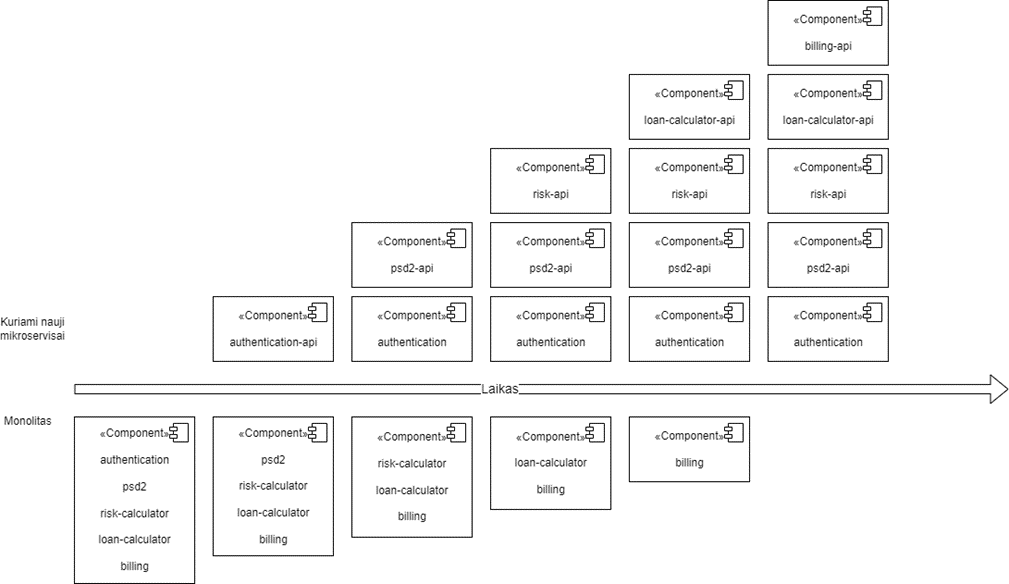
\includegraphics{img/smaugiko-sablonas.png}
    \caption{„Smaugiko“ šablono įgyvendinimas}
    \label{img:smaugiko-sablonas}
\end{figure}

Naujai sukurtiems mikroservisams yra būtina kuo anksčiau priskirti atsakingas komandas. Šios komandos bus atsakingos už tolimesnius mikroservisų darbus, priežiūrą, keitimus, bei teisingos integracijos su dar laikinai naudojamu monolitu užtikrinimą. Taigi prieš visą migraciją privaloma įsivertinti, ar programavimo komandoje pakanka resursų priskirti žmonės specifiniams mikroservisams.


Iš karto gali kilti klausimas: kaip atsirinkti, ką pirmiausia reikia iškelti į naują mikroservisą. Jei šis šablonas yra taikomas pirmą kartą programavimo komandoje, saugiausias variantas būtų pradėti nuo mažiausiai reikšmingo ir/ar mažiausio pagal dydį komponento. Tokiu būdu, komanda įgautų daugiau patirties darbui labiau svarbiems komponentams. Be šito, kiti galimi kandidatai yra \cite{Beh18}:
\begin{itemize}
    \item Komponentai, kurie yra labiausiai užbaigti – turi didžiausią padengimo testais procentą, mažiausiai neužbaigtų techninių darbų. Programavimo komanda tuomet jaustųsi saugiausiai migruodama šį komponentą.
    \item Komponentai, kurie tikėtina, jog plėsis labiausiai. Iškėlus juos į mikroservisus pirmiausia, tikėtina, jog reikės perkelti mažiau kodo, nei tą darbą atliekant vėliau.
    \item Komponentai, kurie dažniausiai kinta dėl besikeičiančių verslo reikalavimų. Tai užtikrintų, jog atliekant verslo reikalaujamus pakeitimus, nereiktų diegti viso monolito, užtektų diegti tik naują mikroservisą.
\end{itemize}

Taigi, šią migravimo strategiją rekomenduojama naudoti tuomet, kai yra aiškiai apibrėžti domenai, arba jei yra galimybė įtraukti verslo atstovus aiškių esminių domenų identifikavimui. Tačiau ši strategija nėra tinkama visiems atvejams. Jos nerekomenduojama naudoti, kai monolitas yra dar itin mažos apimties ir neturi aiškiai apibrėžtų esminių domenų. Priešingu atveju, gali būti brangu sumodeliuoti, kurti bei prižiūrėti naujai sukurtus mikroservisus. Naudojantis šia strategija, atliekamo pertvarkymo darbo laikas tiesiogiai priklauso nuo esamo monolito dydžio. Kuo didesnis monolitas, tuo ilgiau truks jį išskaidyt. Sunkiausia dalis visgi lieka esminių domenų identifikavimas. Taip pat, jei esamame monolite yra didelis kodo padengimas funkciniais testais, tai gali padėti užtikrinti, jog migravimas bus sėkmingas ir reikės atlikti mažiau pilno testavimo rankiniu būdu.

\section{Pilnas sistemos perdarymas}
Nors tai dažnai yra laikoma kraštutine strategija, ją taip pat yra būtina paminėti. Kai esama sistema neatlieka savo verslo funkcijų tinkamai, kai sistemą yra sunku naudoti arba kai sistema yra sukurta naudojant pasenusiomis technologijomis, tada šį monolito migravimo būdą verta apmąstyti \cite{MQO18}.

\subsection{Strategijos aprašymas}
Priežasčių pilnam sistemos perdarymui gali būti keletas. Į šias priežastis yra įtraukta:
\begin{itemize}
    \item Aukštas esamos sistemos palaikymo kaštas \cite{Gli21}. Senoms sistemoms reikia daugiau jas gebančių palaikyti specialistų. Jei monolitas buvo sukurtas su jau pasenusiomis technologijomis, tokių specialistų atrasti gali būti sunku. Jei ir randami šie specialistai, jie bus priskirti prie projekto palaikymo komandos ir tik prižiūrės esamą sistemą, kuri gali veikti klaidingai, arba visai neveikti.
    \item Nepritaikymas esamiems įstatymams. Jei yra išleidžiami nauji įstatymai, kurie apriboja buvusius sistemos panaudos atvejus, esamą monolitinę sistemą pritaikyti pagal tuos įstatymus gali būti labai sudėtinga. Potencialiai, jie gali pakeisti visą verslo logiką, duomenų struktūrą.
    \item Pasenusios technologijos \cite{MQO18}. Surasti specialistus, kurie sugeba palaikyti sistemą, kuri buvo sukurta su senomis technologijomis, gali būti labai sudėtinga. Tokiu atveju sėkmingas verslo užduočių veikimas  yra itin priklausomas nuo specialistų, kurie dirba įmonėje. Idealiu atveju, verslo veiksmingumas neturėtų priklausyti nuo tokių faktorių. Taip pat, senos technologijos reiškia pasenusius saugumo standartus. Sistema tampa mažiau saugi naudoti ir, natūraliai, mažiau patraukli būsimiems ir esamiems vartotojams.
\end{itemize}

Įvertinus esamą sistemą, galima apgalvoti apie sprendimą ją perdaryti ir tuo pačiu pereiti prie mikroservisų architektūros. Bendru atveju, sistemos perdarymas yra vienodai sudėtingas darbas, lyginant su naujos sistemos sukūrimu, taigi yra būtina gauti visos komandos, produkto savininko, projekto vadovo ir kitų suinteresuotųjų asmenų pritarimą sistemos perdarymui. Po įvykdomumo analizės bei reikalavimų surinkimo, belieka įvykdyti sistemos perdarymą. Vykdymas gali būti daromas vienu iš dviejų būdų: „didžiojo sprogimo“ \cite{Ngu11} metodas ir patobulintas perdarymo mechanizmas \cite{MQO18} (angl. enhanced re-engineering mechanism).

\subsection{Strategijos pritaikymas}
„Didžiojo sprogimo“ metodo idėja yra paprasta. Pagrindinis tikslas yra perdaryti visą sistemą vienu metu. Šis metodas įprastai yra pasirenkamas, kai projekto problemą reikia išspręsti kuo greičiau, pvz., pakeisti sistemos architektūrą \cite{Ngu11}. Šis metodas yra itin lankstus, galima atsisakyti nereikalingų sąsajų, galima iškarto prisitaikyti prie naujos diegimo aplinkos. Tačiau šio metodo pritaikymas labai priklauso nuo aktualaus projekto. Metodas netinka labai didelėms sistemoms, nes sunaudojama labai daug resursų. Naudojant šį metodą rizika, jog projektas – perdarymas nepasiseks yra didelė, taigi rekomenduojama pereiti prie sekančios strategijos.
\begin{figure}[H]
    \centering
    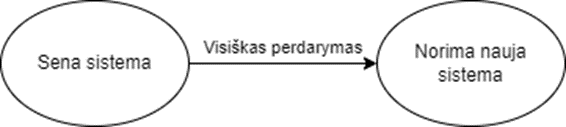
\includegraphics{img/didziojo-sprogimo-metodas.png}
    \caption{„Didžiojo sprogimo“ metodas}
    \label{img:didziojo-sprogimo-metodas}
\end{figure}

Patobulintas perdarymo mechanizmas yra labiau struktūrizuotas procesas, savo žingsniais primenantis klasikinį programų kūrimo procesą. Pirma, yra atliekama įvykdomumo analizė, o tada surenkami reikalavimai naujai sistemai. Turint naujus reikalavimus, pereinama prie programavimo fazės. Atlikus programavimą, atliekamas testavimas, naujų algoritmų palyginimas su sena sistema, naujų technologijų siūlymai ir pakartotinis testavimas. Procesas tęsiasi tol, kol bus pasiektas norimas atnaujinimo lygis. Šis metodas sumažina sistemos perdarymo kompleksiškumą, pagerina naujai perdarytą sistemą ir užtikrina, jog visi reikiami komponentai bus sėkmingai suintegruoti.

\begin{figure}[H]
    \centering
    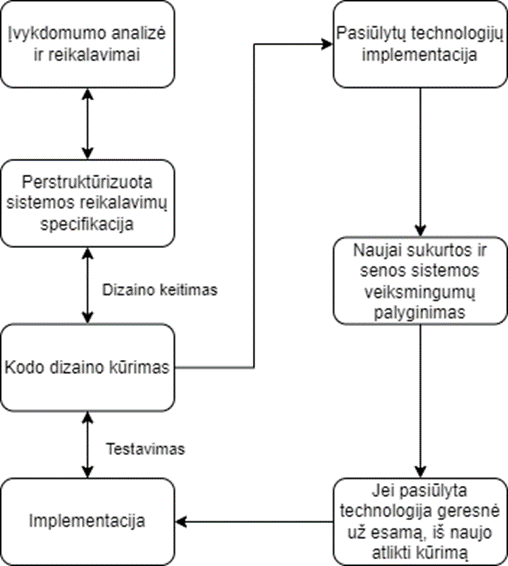
\includegraphics{img/patobulintas-perdarymas.png}
    \caption{Patobulintas perdarymo mechanizmas \cite{MQO18}}
    \label{img:patobulintas-perdarymas}
\end{figure}

Visiškas sistemos perdarymas dažnu atveju yra kraštutinė monolito migravimo priemonė, tačiau tinkamomis sąlygomis, šis metodas atneša daugiau naudos nei tradicinės monolito migravimo strategijos. Pastebėjus didelį kiekį problemų su esama sistema, galima apmąstyti ne tik esamo monolito modernizavimu, bet ir migravimu į mikroservisų architektūrą. Tačiau nedidelis kiekis įmonių yra linkusių pasinaudoti šiuo migravimo metodu, nes jis yra itin ilgai trunkantis ir kainuoja daug resursų \cite{MQO18}. Pastebėta, jog yra modernizavimui skirtų įrankių trūkumas, kuris galėtų paskatinti esamų senų sistemų modernizavimą ir pertvarkymą į mikroservisų architektūrą.

\section{Dekomponavimas naudojant „Mono2Micro”}
Per pastaruosius metus šis metodas pritraukė daug dėmesio. Jo pagalba galima palengvintu būdu atskirti esminius domenus bei juos iškelti į naujus mikroservisus tuo pačiu metu. Naudojantis šiuo įrankiu klaidų tikimybė yra tikėtinai mažesnė, monolito migravimas tampa greitesnis už tradicinius metodus bei turi galimybę paruošti naujus mikroservisus būti naudojamiems debesijoje (angl. cloud computing). Šio darbo rašymo metu, įrankis sėkmingai atlieka migravimo užduotis tik su Java kalba parašytoms programoms, tačiau ateityje yra numatoma apjungti ir kito tipo aplikacijas \cite{KXL+20}.

\subsection{Strategijos aprašymas}
Mono2Micro“ (toliau įrankis) yra dirbtinio intelekto pagalba sukurtas įrankis, kuris padeda pertvarkyti esamą seną sistemą į mikroservisų architektūrą. Įrankis leidžia vartotojui pasirinkti norimus panaudos atvejus ir veikimo metu juos priskirti esančioms klasėms, servisams. Įrankis taip pat atlieka statinę programos analizę ir surenka programos struktūrinę informaciją bei priklausomybes. Šią informaciją tuomet analizuoja dirbtinio intelekto variklis ir sukuria aplikacijos padalinius (angl. partitions) pagal verslo panaudos atvejų, priklausomybių panašumą bei panaudojimą. Sugeneruoti padaliniai yra potencialūs kandidatai naujam mikroservisui. Vartotojas gali peržiūrėti šiuos padalinius, juos redaguoti ar kitaip grupuoti, kad būtų gautas kuo tikslesnis norimas mikroservisas \cite{KXK+21}. Taip pat, kartu su verslo panaudos atvejais, įrankis sugeneruoja natūraliai panašius padalinius. Jie skiriasi tuo, jog nėra analizuojama duomenų priklausomybė. Taip galima supaprastinti duomenų priklausomybes tarp sugeneruotų padalinių.

\begin{figure}[H]
    \centering
    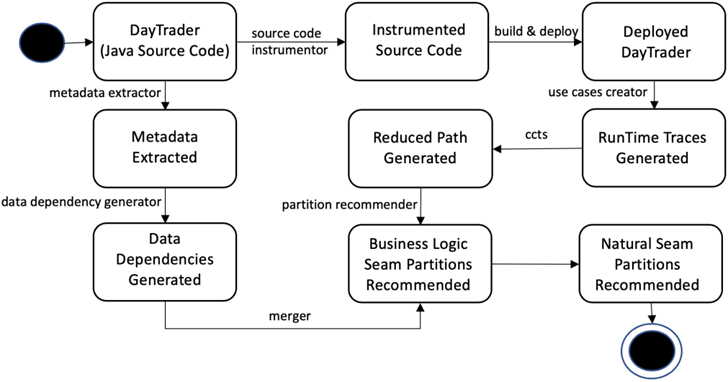
\includegraphics{img/mono-2-micro-veikimas.png}
    \caption{Verslo panaudos atvejų ir natūraliai panašių padalinių generavimas naudojantis „Mono2Micro“ įrankiu \cite{KXL+20}.}
    \label{img:mono-2-micro}
\end{figure}

Kad įrankis sugeneruotų tikslius panaudos atvejus, programa kurią norima pertvarkyti yra paleidžiama. Kai ji pradeda veikti, per vartotojo sąsają būtina atlikti visus panaudos atvejus. Jei kuris nors atvejis bus praleistas, įrankis ieškos daugiau panaudos atvejų funkciniuose testuose. Visa ši informacija yra surenkama į orientuotą grafą (V, E). kur V yra klasės, E yra veikimo metu nustatyti metodų kvietimo sąryšiai tarp klasių \cite{KXL+20}. Sugeneruoto grafo pavyzdys parodomas \ref{img:mono-micro-grafas} pav.

\begin{figure}[H]
    \centering
    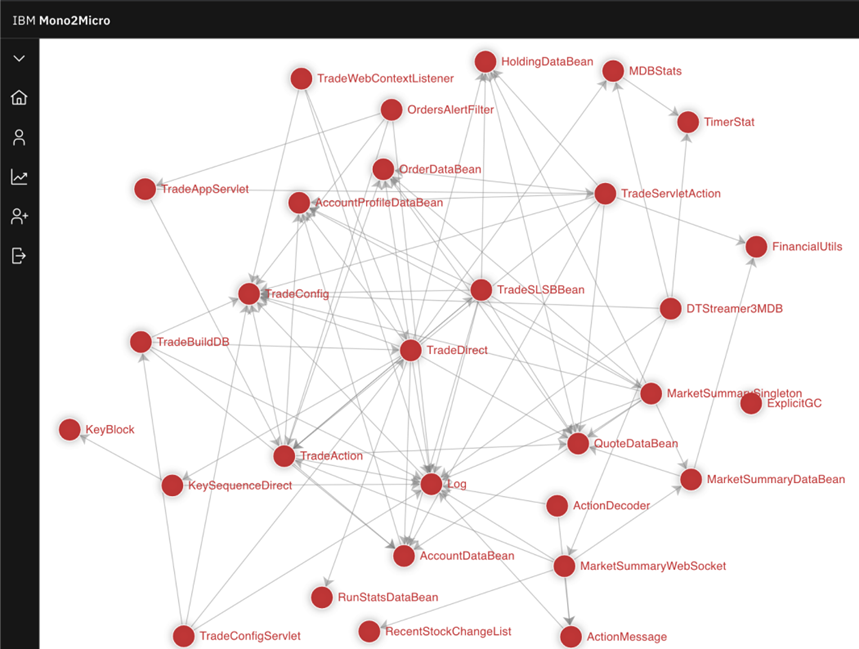
\includegraphics{img/mono-micro-grafas.png}
    \caption{Veikimo metu sugeneruotas orientuotas grafas (V, E), parodantis dinaminius sąryšius tarp klasių \cite{KXL+20}.}
    \label{img:mono-micro-grafas}
\end{figure}

Surinkus visą reikiamą informaciją apie klases ir jų ryšius, įrankis gali pasinaudoti šiais duomenimis bei kvietimo konteksto medžiu (angl. calling-context tree), kad sukurtu padalinių rekomendacijas. Turint norimą padalinių skaičių k ir klasių aibę C = {c1, c2, ..., cn} galima sugrupuoti klases pasinaudojant šia panašumo formule \cite{KXL+20}.

\begin{equation}\label{eq:panasumo-formule}
    Sim_{i,j} = \frac{\sum_{m=o}^{n_{i}}\sum_{n=0}^{n_{j}}S(c_{im},C_{jn})}{\left| C_{i} \right|\left| C_{j} \right|}
\end{equation}

Panašumo dydis yra apskaičiuojamas remiantis tiesioginiais ir netiesioginiais kvietimų ryšiais tarp klasių $c_{i}$ ir $c_{j}$. Tiesioginio kvietimo ryšys egzistuoja tik tuomet, kai ryšys tarp klasių $c_{i}$ ir $c_{j}$ egzistuoja kvietimo konteksto medyje briauna $(c_{i}, c_{j})$. Netiesioginio kvietimo ryšys tarp klasių $c_{i}$ ir $c_{j}$ egzistuoja tik tuomet, jei konteksto kvietimo medyje egzistuoja kelias $(c_{i}, c_{2}, ..., c_{p}, c_{j}), p > 1$.

Kai yra sugeneruojami padaliniai pagal panaudos atvejų panašumą, įrankis juos sujungia pagal natūralų panašumą. Jei klasės ci ir cj turi ryšių, jos yra priskiriamos vienam padaliniui. Tokiu būdu pereinama per visas visų padalinių klases ir gaunamas optimalus natūraliai panašių padalinių skaičius.

\subsection{Strategijos pritaikymas}
Šiai strategijai išbandyti naudojama populiari „IBM“ sukurta etaloninė programa „DayTrader“ \cite{IBM15}. Tai yra elektroninė akcijų pirkimo ir pardavimo programa. Ji leidžia vartotojui prisijungti, peržiūrėti savo profilį, peržiūrėti esamas akcijas, jų kainas bei kainų istoriją, pirkti bei parduoti akcijas. Joje yra 112 klasių ir 964 metodų. Kodo padengimas funkciniais testais – padengta  66 \% klasių, 44 \% metodų. Pasinaudojus įrankiu ir nurodžius padalinių skaičių $k = 7$ gauname rekomenduojamus 3 padalinius $p_{1}, p_{2}, p_{3}$.

\begin{figure}[H]
    \centering
    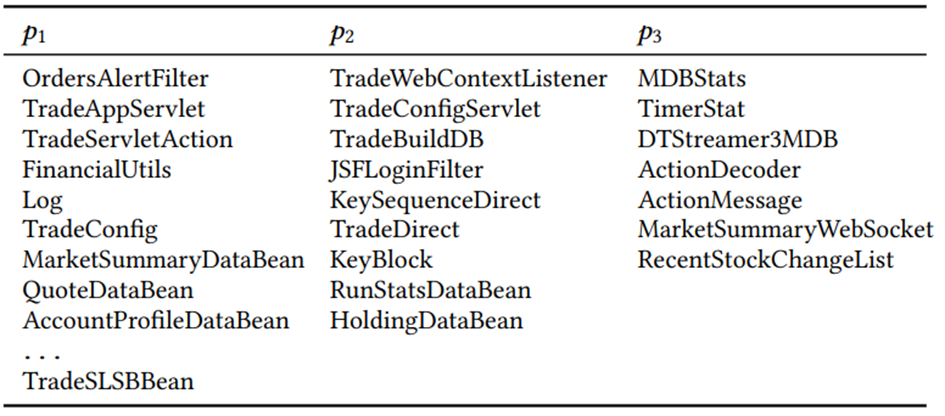
\includegraphics{img/mono-micro-padaliniai.png}
    \caption{Sugeneruoti padaliniai „DayTrader“ programai, kai $k = 7$, \cite{KXK+21}}
    \label{img:mono-micro-padaliniai}
\end{figure}

Padalinyje $p_{1}$ yra priskiriamos klasės, susijusios su akcijų pirkimo ir pardavimo funkcionalumu, $p_{2}$ yra priskiriamos klasės, susijusios su duomenų bazės operacijomis, o $p_{3}$ yra priskiriamos klasės susijusios su įvairių pranešimų siuntimu. Šie padaliniai buvo suskirstyti pagal panaudos atvejus ir jie nėra glaudžiai susiję su verslo moduliais pasinaudojant įrankio padalinių sujungėju. Parodžius šiuos rezultatus programinės įrangos architektams, kurie yra susipažinę su šia programa, jie patvirtino, jog šie „Mono2Micro“ sugeneruoti mikroservisų patarimai yra logiški ir prasmingi \cite{KXL+20}.

„Mono2Micro“ puikiai tinka sugeneruoti esamo Java EE monolito pertvarkymo rekomendacijoms. Šis įrankis yra itin lankstus, suteikiantis daug patarimų ir rekomendacijų, ir parodė, jog veikia gerai su vidutinio dydžio Java Spring programomis \cite{San21}. Taip pat galima pastebėti, jog šis įrankis gali būti naudojamas ne tik monolito paruošimui mikroservisų architektūrai, bet ir patikrinti, ar monolitą tikrai verta skaldyti į atskirus mikroservisus. Jei gaunamas rekomenduotinų padalinių skaičius yra nedidelis (pvz., 2), tai verta pamąstyti, ar apsimoka skirti laiko ir resursų šiam sudėtingam darbui. Nors šis įrankis šiuo metu veikia tik su Java EE programomis, tikėtina, jog jis ateityje palengvins ir kitokio tipo programų pertvarkymą.

\sectionnonum{Išvados}
\begin{itemize}
    \item Monolito migravimas į mikroservisų architektūrą yra sudėtingas ir daug planavimo reikalaujantis darbas. Ne visus monolitus reikia pertvarkyti į naują architektūrą, tačiau privaloma kurti monolitus prisiminant, jog jie gali plėstis ir bus privaloma juos pertvarkyti ateityje.
    \item Monolito pertvarkymas yra visiškai techninė užduotis, taigi privaloma gauti produkto savininko sutikimą planuojamam pertvarkymui.
    \item Esminių domenų identifikavimas yra daug laiko atimantis darbas, tačiau itin svarbus. Jei tik įmanoma, į šį procesą būtina įtraukti verslo atstovus, sistemos programavimo pradininkus bei kitas šalis, kurios yra geriausiai susipažinusios su pertvarkoma sistema.
    \item Dekomponavimas pagal domenus yra klasikinis migravimo būdas, tačiau yra itin svarbu turėti aiškiai apibrėžtus esminius domenus. Jei esminiai domenai nebus tinkamai apibrėžti, gauta mikroservisų architektūra gali atnešti daug nuostolių.
    \item Dekomponavimas pagal domenus yra statinis migravimo būdas, trunkantis daugiausia laiko. Kad ši užduotis būtų kuo paprastesnė, privaloma nuo pat monolito kūrimo pradžios laikytis gerųjų programavimo praktikų: logiški klasių, metodų, paketų pavadinimai, kodo padengimas testais, loginis komponentų grupavimas.
    \item Visiškas sistemos perdarymas yra daugiausiai kainuojantis metodas, tačiau verta apmąstyti šią strategiją, nes ji gali atnešti daugiau naudos nei kiti minėti būdai. Šią strategiją, ar jos dalį, rekomenduojama panaudoti kartu su kitais migravimo būdais.
    \item „Mono2Micro“ įrankis puikiai veikia identifikuojant esminius domenus, arba juos sugrupuoti pagal natūralų panašumą. Tačiau kad šis įrankis veiktų gerai, verta turėti monolitą, kuris turi ne tik išbaigtą vartotojo sąsają, bet ir didelį kodo padengimą funkciniais testais.
    \item Empiriniu būdu nustatyta, jog apjungus dekomponavimo pagal domenus ir „Mono2Micro“ įrankio strategijas, migravimas tampa labai supaprastintu.
    \item Bakalauro baigiamajame darbe bus daugiau tiriama „Mono2Micro“ ir dekomponavimo pagal domenus strategijų praktiniai privalumai ir trūkumai. Bus tiriama, kaip „Mono2Micro“ veikia su skirtingo dydžio programomis, su skirtingais kodo padengimais testais bei kitais aktualiais parametrais.
\end{itemize}

\printbibliography[heading=bibintoc]  % Šaltinių sąraše abėcėlės tvarka išdėstomi darbe panaudotų
% (cituotų, perfrazuotų ar bent paminėtų) mokslo leidinių, kitokių publikacijų
% bibliografiniai aprašai. Aprašai pateikiami netransliteruoti.

\end{document}